\documentclass[11pt, oneside]{article}
\usepackage[letterpaper, margin=2cm]{geometry}
\usepackage{AERE546}
\usepackage{xspace}

\begin{document}
\noindent \textbf{\Large{Caleb Logemann \\
AER E 546 Fluid Mechanics and Heat Transfer I \\
Homework 4
}}

%\lstinputlisting[language=MATLAB]{H01_23.m}
\begin{enumerate}
  \item % #1
    The laser heating in the second problem of homework 3 should probably be
    modeled as a localized hot-spot in two dimensions - assuming that the slab
    is thin, so it is heated uniformly across its thickness.
    Solve the (non-dimensional) diffusion equation
    \[
      \pd{T}{t} = \nabla^2 T \qquad \nabla^2 = \pd[2]{}{x} + \pd[2]{}{y}
    \]
    in the square region $0 \le x, y \le 1$.
    Form the semi discrete equations and integrate in time by RK2.
    Choose a suitable $\Delta t$.
    Submit only the algorithm part of your code.

    The walls are kept cool, i.e. $T = 0$ on the boundaries.
    The initial hot spot is represented by
    \[
      T(x, y) = \frac{1}{\pi \sigma^2} e^{-r^2/\sigma^2} \qquad r^2 = (x - 0.25)^2 + (y - 0.25)^2, \sigma = 0.1
    \]
    \begin{itemize}
      \item Let $Nx = Ny = 201$. Provide a plot of contour lines of the
        solution at $t = 0.02$ and $t = 0.1$.

      \item How long $(t = ??)$ must you wait for the maximum temperature to
        drop to $1\%$ of its intial value?
    \end{itemize}

    The following function runs the second order Runge-Kutta method for any
    given right hand side operator.
    This is the same method that was used in an earlier homework.
    \lstinputlisting[language=MATLAB]{RK2.m}
    The following function implements the right hand side for the 2D heat operator.
    \lstinputlisting[language=MATLAB]{HeatRHS2D.m}
    %The following script now uses both of these functions to actually solve the problem
    %\lstinputlisting[language=MATLAB, lastline=42]{H04.m}

    Using both of these function the following images can be produced.
    These show the temperature profile at $t = .02$ and $.1$.
    Note that the overall temperature is much less at $t = .1$ because most of
    the energy has diffused out through the boundaries.
    \begin{center}
      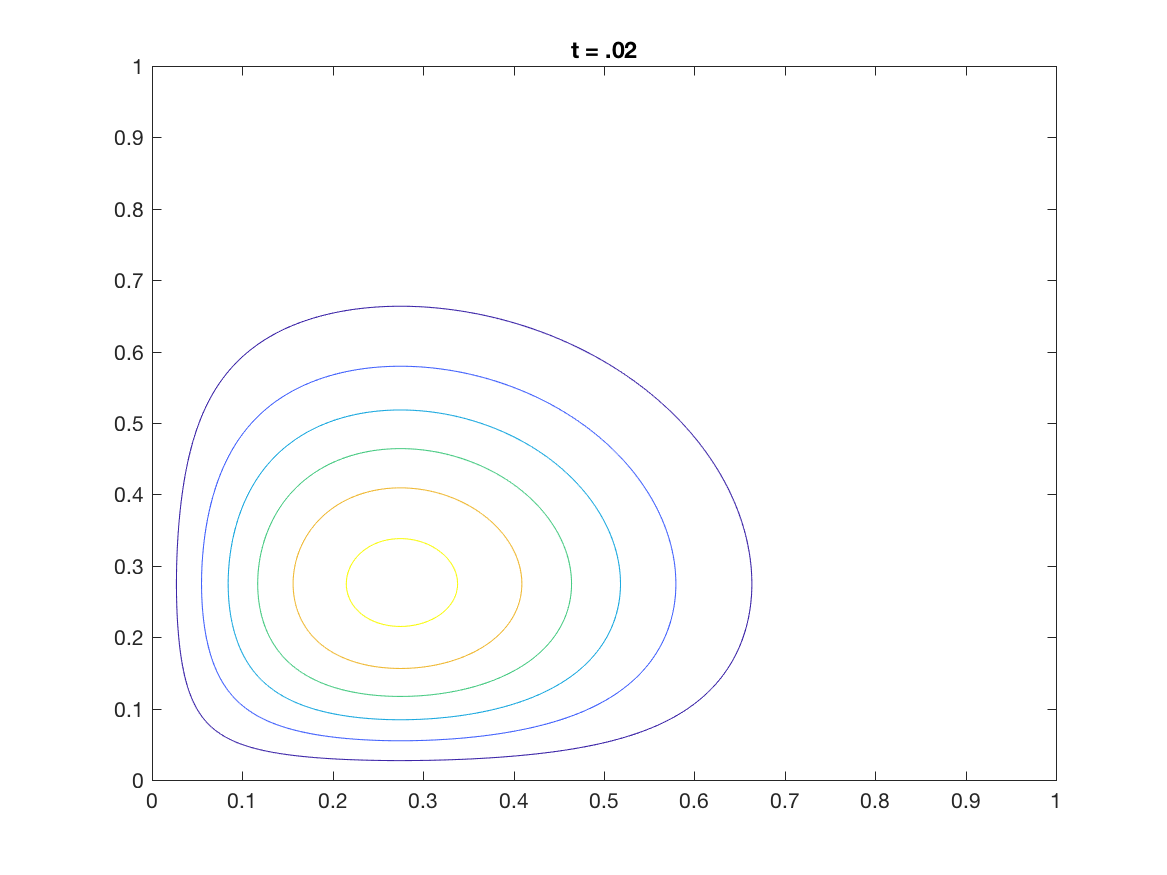
\includegraphics[width=0.45\textwidth]{Figures/04_01.png}
      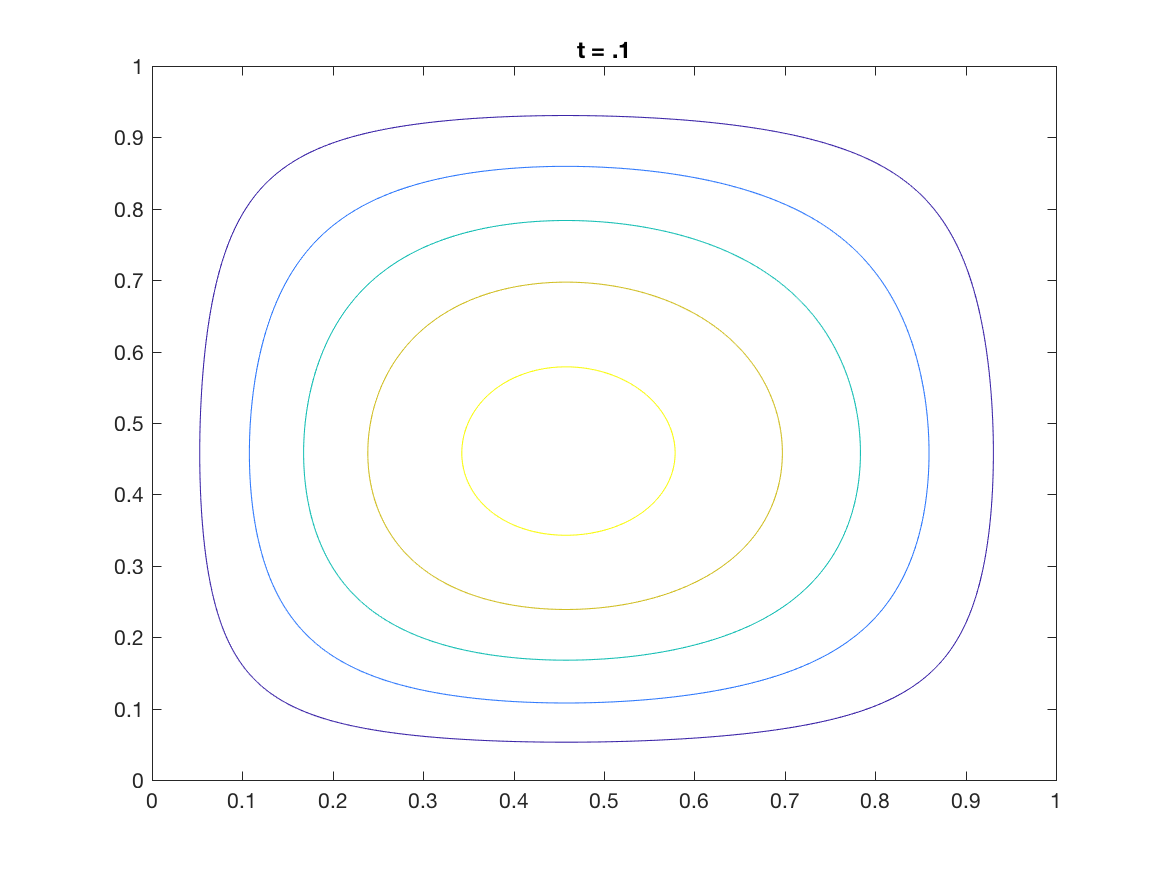
\includegraphics[width=0.45\textwidth]{Figures/04_02.png}
    \end{center}

    Taking the maximum after each time step we see that
    at $t = 0.092$ the maximum value just drops past 1\% of the initial
    maximum value.
  \item % #2 Done
    Explain why ADI is called approximate factorization - i.e. make sure you
    understand the formal basis for the method.

    Use the ADI scheme with Euler implicit time-stepping to solve the same heat
    equation, as in the previous problem, in the same square, $0 \le x, y \le 1$.
    But now, initially $T = 0$ everywhere, except on the lower wall.
    The boundary conditions are
    \begin{gather*}
      T = \sin[2]{2 \pi x} \text{ on } y = 0; 0 \le x \le 1 \\
      T = 0 \text{ on } x = 0 \text{ and } x = 1; 0 \le y \le 1 \\
      T = 0 \text{ on } y = 1; 0 \le x \le 1
    \end{gather*}
    Integrate to $t = 0.25$ and plot temperature contours at
    $t = 0.002, 0.01, 0.04$ and $t = 0.1$.
    Provide a line plot of $T(1/2, 1/2)$ versus $t$; has the solution converged
    to steady state?
    If so, what equation has been solved?
    Provide the algorithm part of your code - with brief comment lines, showing
    how you implemented ADI.

    ADI is called an approximate factorization as it is making the following
    approximation
    \[
      \p{1 - \pd[2]{}{x} - \pd[2]{}{y}} \approx \p{1 - \pd[2]{}{x}}\p{1 - \pd[2]{}{y}}
    \]
    This operator does not exactly factor like this, but it is accurate to $\Delta x^4$
    so the factorization is approximately correct.

    The following function now implements the ADI method.
    \lstinputlisting[language=MATLAB]{ADI.m}
    The following script now uses the previous function to solve the heat
    equation with the given boundary conditions and initial values.
    \lstinputlisting[language=MATLAB, lastline=108, firstline=84]{H04.m}
    The following images are produced.
    \begin{center}
      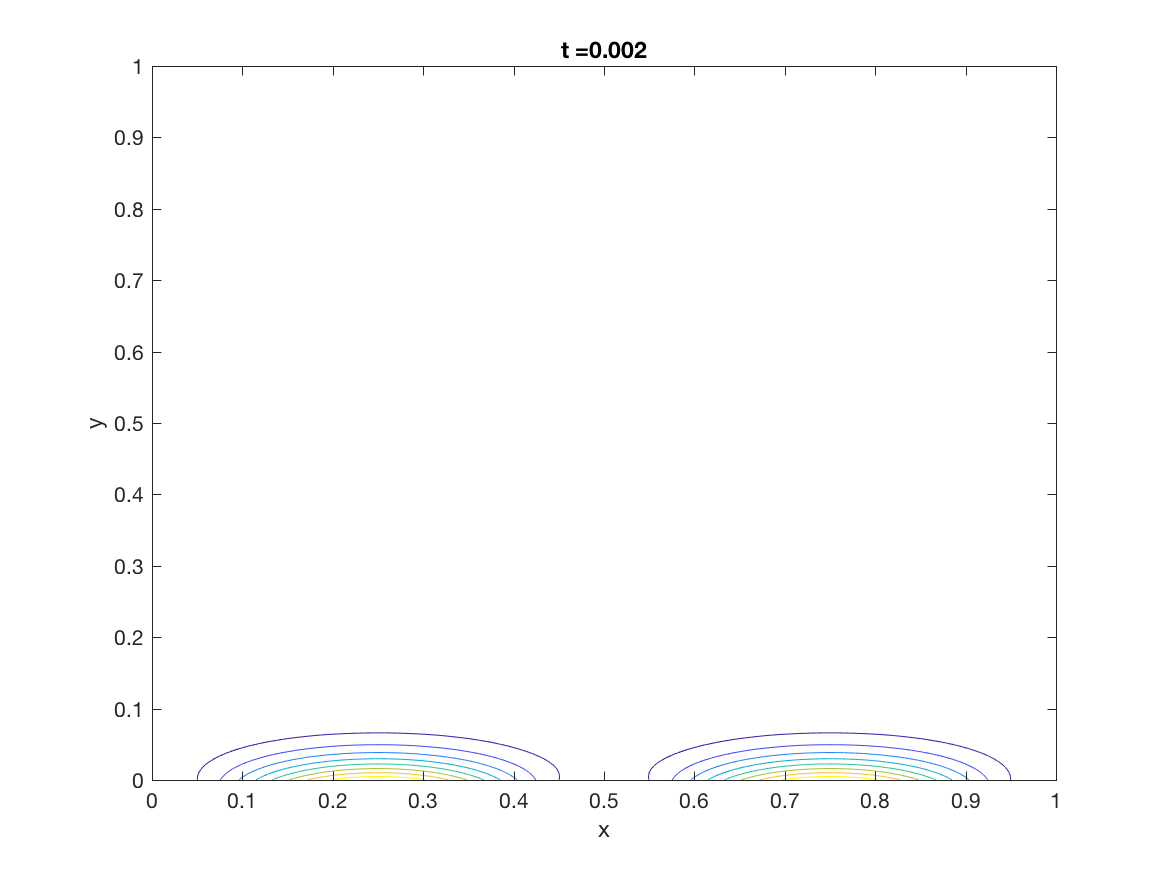
\includegraphics[width=0.45\textwidth]{Figures/04_03.png}
      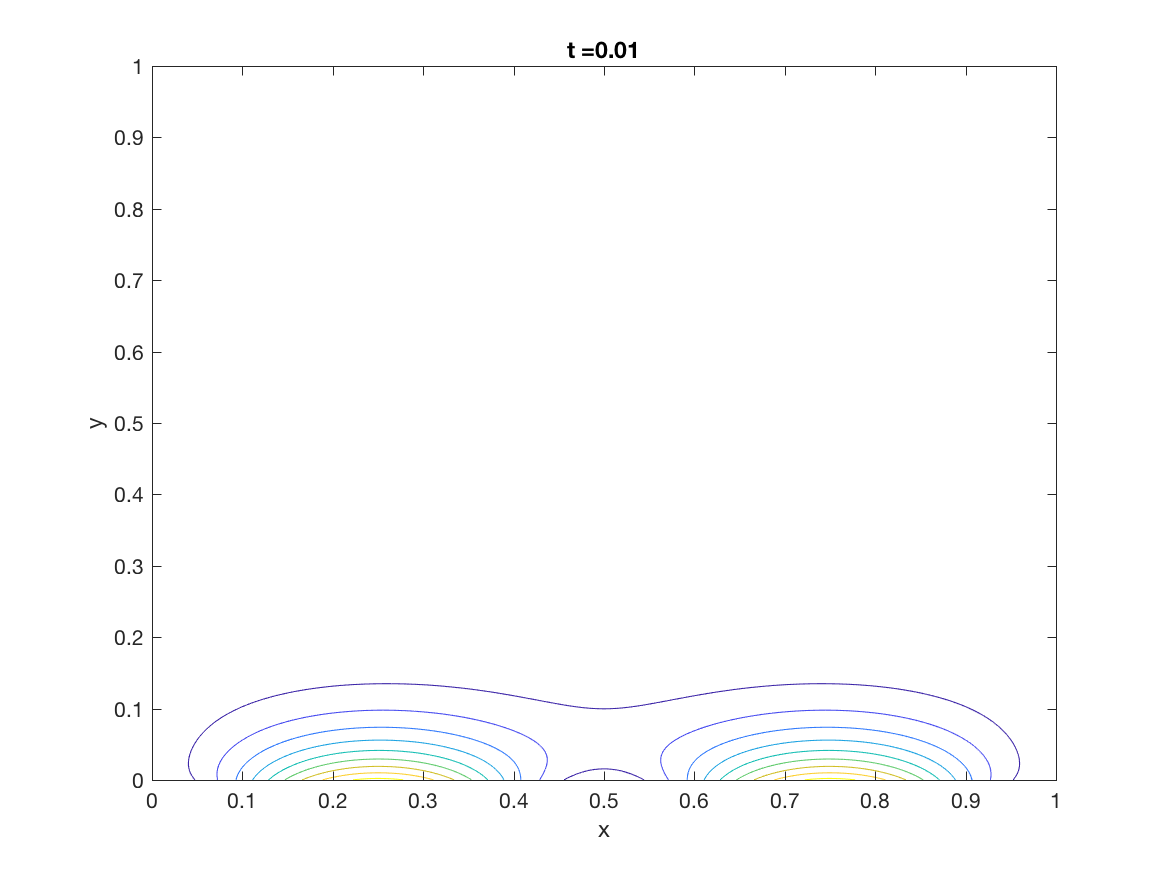
\includegraphics[width=0.45\textwidth]{Figures/04_04.png}
      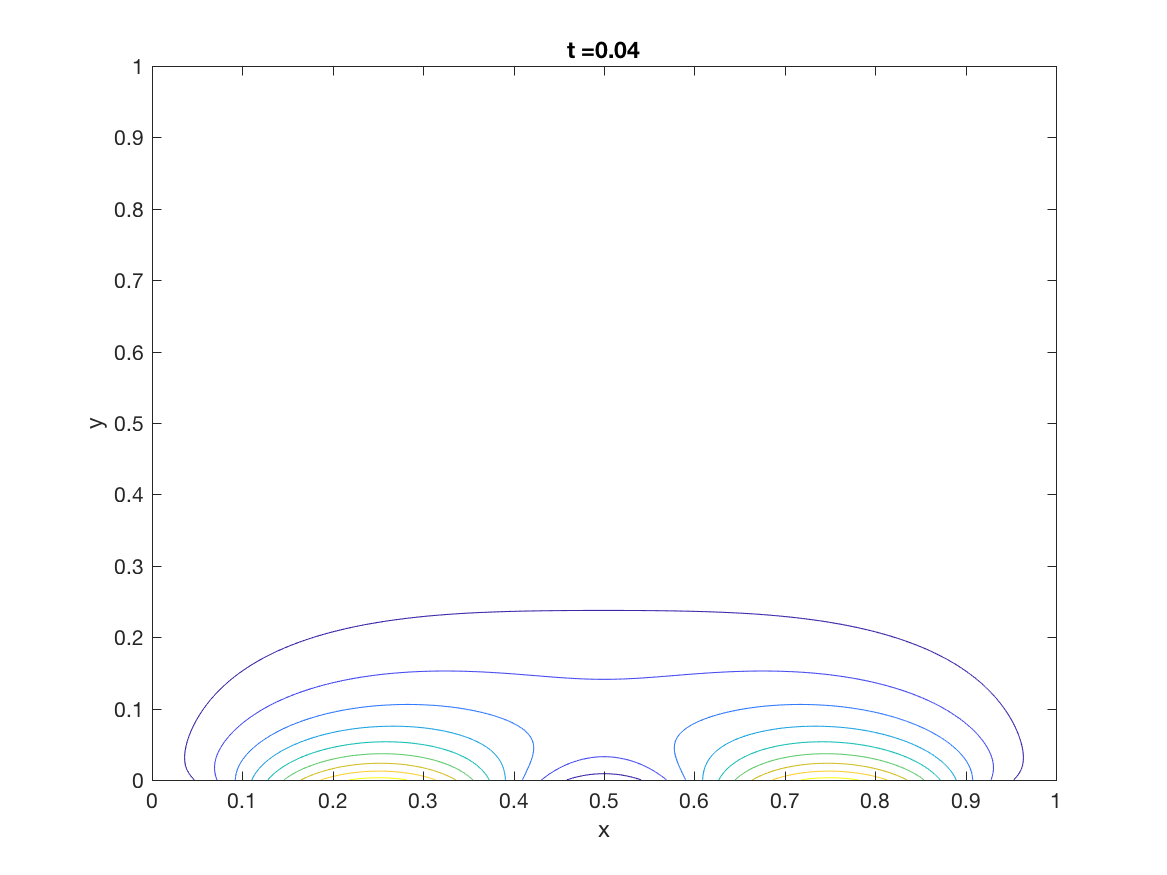
\includegraphics[width=0.45\textwidth]{Figures/04_05.png}
      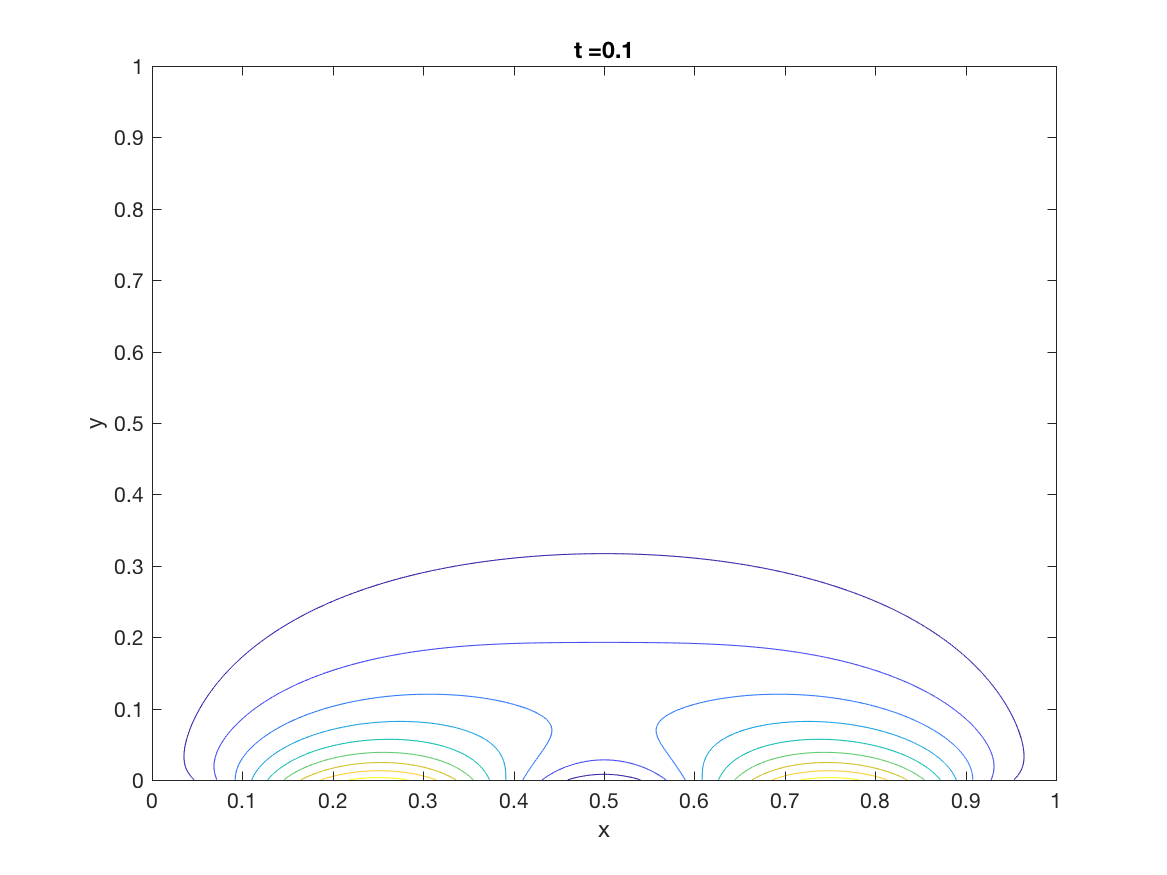
\includegraphics[width=0.45\textwidth]{Figures/04_06.png}
      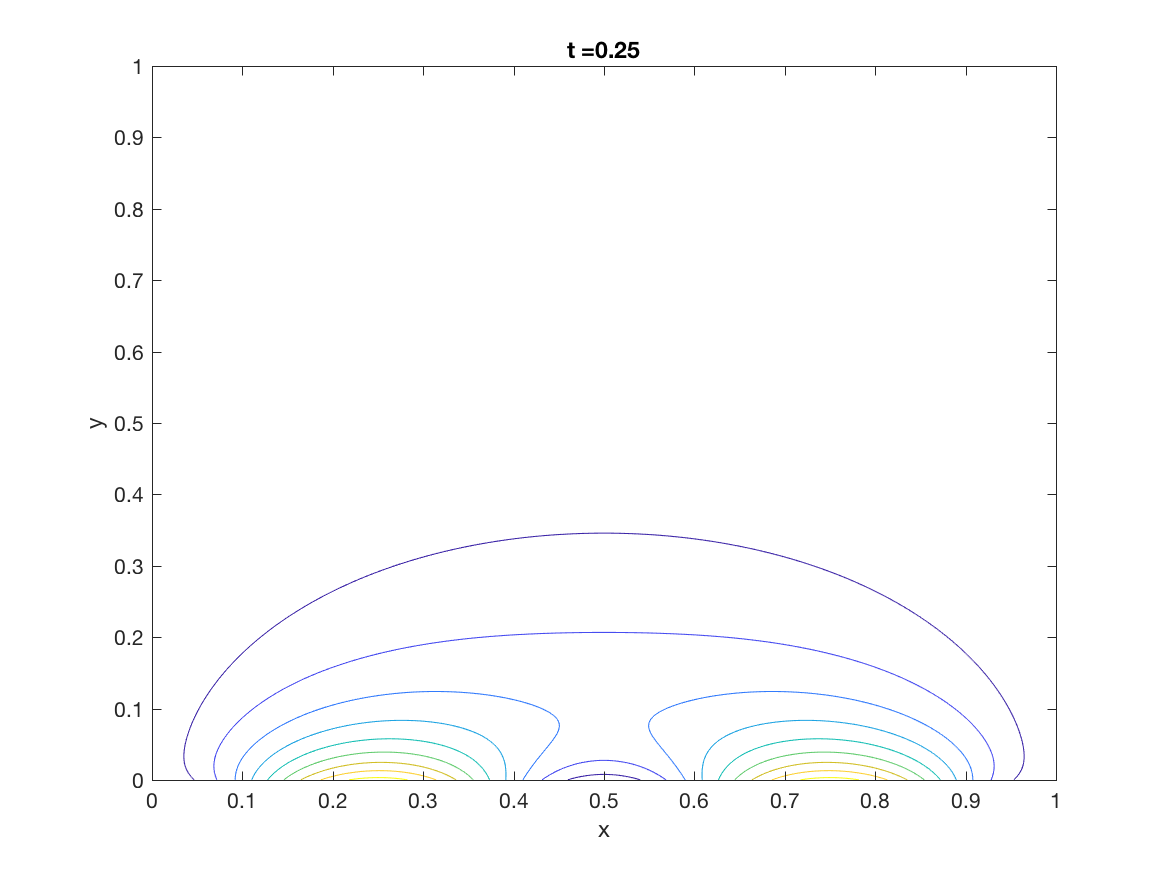
\includegraphics[width=0.45\textwidth]{Figures/04_07.png}
    \end{center}
    The following is a graph of the temperature at $(0.5, 0.5)$ over
    the course of the simulation.
    As you can see the temperature is approaching a steady state.
    This means that the final solution is actually a solution to the
    steady state elliptic problem
    \[
      \nabla^2 T = 0.
    \]
    \begin{center}
      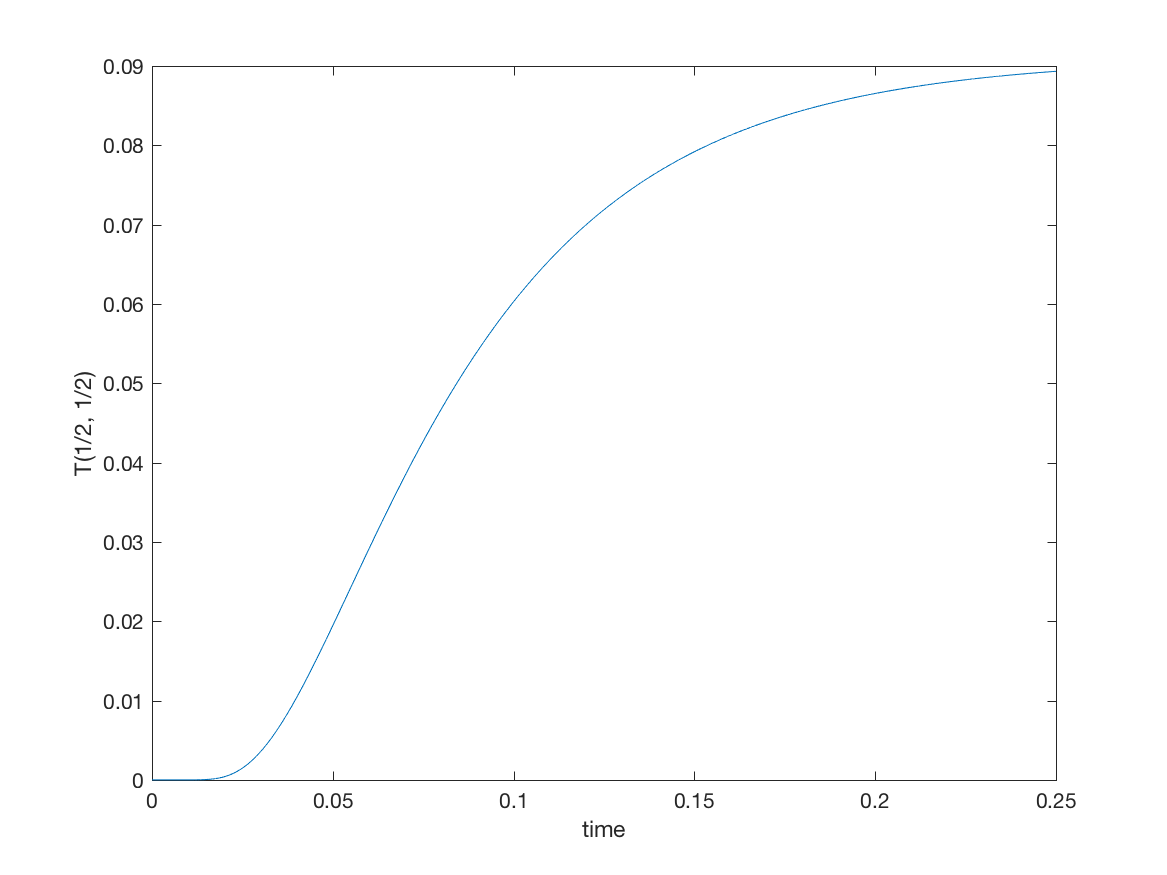
\includegraphics[scale=0.5]{Figures/04_08.png}
    \end{center}

\end{enumerate}
\end{document}
